\documentclass[11pt,a4paper]{article}
\usepackage[a4paper,margin=2.3cm]{geometry}
\usepackage{amsmath,amssymb,amsthm}
\usepackage{booktabs}
\usepackage{graphicx}
\usepackage{float}
\usepackage[numbers]{natbib}
\usepackage{hyperref}
\usepackage{xcolor}
\usepackage{enumitem}
\usepackage{array}
\usepackage{caption}
\usepackage{microtype}
\usepackage{url}
\graphicspath{{figures/peak_shaving_final_20260714/}{figures/}{./}}
\hypersetup{colorlinks=true,linkcolor=blue,citecolor=blue,urlcolor=blue}
\captionsetup{font=small,skip=4pt}
\setlength{\emergencystretch}{3em}

\newtheorem{proposition}{Proposition}
\newcommand{\T}{\mathcal{T}}
\newcommand{\M}{\mathcal{M}}
\newcommand{\Channels}{\mathcal{C}}
\newcommand{\Sset}{\mathcal{S}}
\DeclareMathOperator*{\argmax}{arg\,max}

\title{\textbf{Time-of-use pricing for fixed-capacity inference services: a simulation of temporal load shifting and provider substitution}}
\author{Anonymous Author}
\date{}

\begin{document}
\maketitle
% Generated from machine-readable submission artifacts. Do not edit.
\newcommand{\AggregatePeakChangePercent}{-12.50}
\newcommand{\AggregatePeakReductionPercent}{12.50}
\newcommand{\DynamicAggregatePeak}{196.903}
\newcommand{\DynamicColSupportCount}{26}
\newcommand{\DynamicEvaluatedPairs}{81,276}
\newcommand{\DynamicGridRegret}{1.14e-13}
\newcommand{\DynamicIntermediaryProfit}{345.410}
\newcommand{\DynamicMarketProfit}{1922.935}
\newcommand{\DynamicMaximumUtilisation}{1.223}
\newcommand{\DynamicMinimumQoS}{0.959}
\newcommand{\DynamicMovedFraction}{0.327}
\newcommand{\DynamicPeakToAverage}{1.432}
\newcommand{\DynamicProviderAProfit}{835.666}
\newcommand{\DynamicProviderBProfit}{741.859}
\newcommand{\DynamicRelativeGridRegret}{1.36e-16}
\newcommand{\DynamicRowSupportCount}{26}
\newcommand{\IntermediaryProfitChangePercent}{7.78}
\newcommand{\MarketProfitChangePercent}{2.23}
\newcommand{\MaximumJointResidual}{1e-09}
\newcommand{\MaximumUtilisationChangePercent}{-10.84}
\newcommand{\MaximumUtilisationReductionPercent}{10.84}
\newcommand{\MinimumQoSChange}{0.057}
\newcommand{\MovedFractionChange}{0.0137}
\newcommand{\ProviderAProfitChangePercent}{-1.08}
\newcommand{\ProviderBProfitChangePercent}{3.65}
\newcommand{\ProviderCandidateCount}{1576}
\newcommand{\UniformAggregatePeak}{225.043}
\newcommand{\UniformCandidateCount}{800}
\newcommand{\UniformIntermediaryProfit}{320.483}
\newcommand{\UniformMarketProfit}{1880.935}
\newcommand{\UniformMaximumUtilisation}{1.371}
\newcommand{\UniformMinimumQoS}{0.901}
\newcommand{\UniformMovedFraction}{0.313}
\newcommand{\UniformPeakToAverage}{1.637}
\newcommand{\UniformProviderAProfit}{844.748}
\newcommand{\UniformProviderBProfit}{715.704}


\begin{abstract}
Time-of-use pricing offers a market-level mechanism for relieving congestion in inference services, but the observed response can mix temporal load shifting with substitution across providers and purchase channels. We develop a conserved-demand simulation with two capacity-asymmetric providers, direct access, and an application programming interface intermediary. Origin--destination flows describe temporal movement before users choose a purchase channel, and provider load, intermediary routing, and quality of service (QoS) are solved as a joint fixed point. The intraday load shape is anchored by 59 complete days from the 1,429,737-record BurstGPT trace, and controlled vLLM measurements determine the shape of the QoS function. Providers choose from a declared set of \ProviderCandidateCount{} bounded linear price rules; the uniform-price comparison uses \UniformCandidateCount{} zero-slope rules over the full base-price domain. The intermediary response is obtained by bounded multistart optimization over a continuous three-parameter pricing and routing rule. We compute a mixed equilibrium of this declared finite game from complementarity conditions and check it against every candidate deviation. Relative to the equilibrium under the uniform-price restriction, time-varying prices reduce the expected aggregate peak by \AggregatePeakReductionPercent\% and the expected maximum provider utilization by \MaximumUtilisationReductionPercent\%. Expected minimum QoS rises from \UniformMinimumQoS{} to \DynamicMinimumQoS{}, while aggregate market-side profit changes by \MarketProfitChangePercent\%. The evidence supports a service-quality interpretation under the stated synthetic economic calibration, with scope limited to simulation rather than a production forecast or a continuous-space equilibrium proof.
\end{abstract}

\noindent\textbf{Keywords:} simulation modelling; inference services; time-of-use pricing; demand response; quality of service; mixed-strategy equilibrium; model verification

\section{Introduction}
\label{sec:introduction}

Online large language model (LLM) services operate under finite graphics processing unit (GPU) capacity. Request load varies within the day, whereas short-run capacity is difficult to adjust at the same pace. Local overload can increase time to first token (TTFT), queueing delay, and service-level objective failures. Serving systems address these effects through batching, memory management, scheduling, and disaggregation \cite{yu2022orca,kwon2023pagedattention,agrawal2024sarathiserve,patel2024splitwise,zhong2024distserve}. These controls act after requests have reached a platform.

Pricing acts earlier in the service process. A provider can raise prices in busy periods and lower them when capacity is less utilized, giving flexible workloads an incentive to change execution time. This idea is closely related to electricity demand response \cite{schweppe1988spot,borenstein2005long,albadi2008summary,faruqui2010household,siano2014demand}. Both settings combine variable demand with a capacity limit. Inference markets add a second response because requests can also change provider or purchase channel.

These two responses require separate measurement. A lower maximum provider utilization may arise from traffic moving between providers, even when total demand in that period is unchanged. We call movement across periods temporal load shifting and changes in channel or provider spatial substitution. A peak-utilization measure alone therefore cannot identify which response produced a QoS change.

Recent studies consider inference cost, menu pricing, strategic routing, GPU scaling, and token-based capacity control \cite{demirer2025emerging,bergemann2025menu,guo2026prillm,yan2026stackelberg,cunningham2026token}. Serving simulators and workload traces provide a separate account of system behavior \cite{agrawal2024vidur,wang2025burstgpt}. Taken separately, these streams leave open whether a price-induced load change comes from rescheduling, channel substitution, market exit, or demand growth. A market simulation must track native arrivals, destination periods, purchase channels, intermediary routing, congestion, and payments in one model.

We study whether bounded linear time-of-use price rules can protect QoS when temporal and spatial responses are represented explicitly. Total demand is fixed. Origin--destination (OD) flows conserve each request type before users choose a channel. The application programming interface (API) intermediary then routes its demand using provider prices and QoS. Provider load changes QoS, which feeds back into user choice and routing.

The main contribution is a simulation model that separates aggregate peak reduction from spatial substitution while retaining this feedback. Providers play a finite game over a declared set of bounded price rules. The intermediary optimizes a three-parameter price-and-routing rule on bounded domains, and the market state is computed as a coupled fixed point. The analysis uses an observed intraday load shape and a measured QoS curve, while the economic parameters remain synthetic. Under this design, time-varying prices improve the congestion and QoS measures, while aggregate market-side profit rises in the main case. The conclusion is a modeled service-quality effect under a stated calibration, rather than a production forecast.

\section{Related work}
\label{sec:related}

\subsection{Electricity pricing as the modelling foundation}

Electricity pricing is the clearest established example of price-induced temporal demand response. Spot and real-time prices connect short-run scarcity with the timing of consumption \cite{schweppe1988spot,borenstein2005long}. Time-of-use tariffs use fixed period blocks, whereas critical-peak and real-time tariffs expose users to sharper scarcity signals. Reviews of demand-response programs show that user flexibility and tariff design jointly determine the observed peak change \cite{albadi2008summary,siano2014demand}.

Empirical electricity studies also show why the response must be measured carefully. Faruqui and Sergici review 15 household experiments and report peak reductions of 3--6\% for time-of-use tariffs and 13--20\% for critical-peak pricing \cite{faruqui2010household}. Allcott reports lower peak use under hourly pricing without a matching rise in average off-peak use \cite{allcott2011rethinking}. A lower peak can reflect conservation, rescheduling, or both. Our model isolates rescheduling by conserving each origin-period demand mass.

Utility-based models link prices with flexible consumption. Samadi et al. derive real-time prices from utility maximization, and Yang et al. represent time-of-use pricing as a game \cite{samadi2010optimal,yang2013game}. Recent work also uses game theory to vary on-peak and shoulder-period prices across users according to their load contribution \cite{elafifi2024game}. Stackelberg models place a utility or retailer above responding users \cite{yu2016supply,srinivasan2017game}. A recent virtual-power-plant model adds a distribution-system operator and formulates the resulting three-level interaction as a fixed-point problem \cite{wang2026hierarchical}. These hierarchies are relevant to inference services because providers announce prices before demand is allocated. Their constraints and outcomes remain specific to electricity dispatch. They do not combine two competing inference providers, an API intermediary, direct purchase, and endogenous service quality in one model.

Reinforcement learning has also been used to learn dynamic tariffs when demand response is uncertain \cite{vazquez2019reinforcement,ismail2023dynamic}. Fraija et al. adjust a price-generator rule under market and capacity constraints \cite{fraija2024dynamic}. These methods can search sequential pricing policies, but they do not by themselves show that competing providers have reached a Nash equilibrium. Our question concerns strategic stability and unilateral deviations. We retain interpretable linear price rules and solve the provider game directly.

The transfer from electricity to inference is partial. Deferrable inference jobs can respond to time-varying prices in a similar way to shiftable electrical loads. Interactive or deadline-sensitive requests have much less temporal flexibility. Inference requests can also change provider without changing execution time. The present model retains the temporal logic of electricity pricing and adds this provider-substitution response.

\subsection{Inference serving, workload measurement, and market models}

Inference-serving research mainly studies decisions inside the computing system. Clipper and Clockwork target predictable low-latency inference \cite{crankshaw2017clipper,gujarati2020clockwork}. Orca, vLLM, Sarathi-Serve, Splitwise, and DistServe improve batching, memory use, or phase scheduling \cite{yu2022orca,kwon2023pagedattention,agrawal2024sarathiserve,patel2024splitwise,zhong2024distserve}. Vidur provides a large-scale simulation framework for LLM serving \cite{agrawal2024vidur}. These studies show that latency and goodput depend on local load, but demand is usually an input rather than a price-responsive outcome.

Workload traces improve the empirical basis of such simulations. BurstGPT contains Azure OpenAI request records and documents bursty arrival and token patterns \cite{wang2025burstgpt}. We use its intraday token profile as a load-shape anchor. Because the trace does not include experimental price variation, the utility price coefficients and migration cost remain part of the synthetic calibration.

Recent market studies consider inference cost, contract design, routing, and token allocation. Work on the market for intelligence and LLM menu pricing examines supply and demand at the market level \cite{demirer2025emerging,bergemann2025menu}. PriLLM formulates a data-calibrated Stackelberg routing and pricing game \cite{guo2026prillm}. Other models study GPU platform pricing and token allocation \cite{yan2026stackelberg,cunningham2026token}. These studies introduce strategic behavior, but they do not separate OD time movement from within-period provider substitution in the form used here.

\subsection{Model positioning and numerical evidence}

Congestion pricing and revenue management explain how prices allocate limited capacity over time \cite{vickrey1969congestion,arnott1990bottleneck,gallego1994dynamic,elmaghraby2003dynamic}. Discrete-choice models provide a basis for price-sensitive channel and time choices \cite{mcfadden1974conditional,anderson1992discrete,train2009discrete}. Platform models explain how an intermediary can affect allocation between users and providers \cite{rochet2003platform}. Our simulation combines these elements in a small market whose flows and payments can be checked directly.

Simulation studies also need to distinguish model verification from validation against an observed system \cite{sargent2013verification}. We use verification for conservation, accounting, numerical residuals, and equilibrium regret. BurstGPT and the vLLM experiment provide empirical inputs, but they do not validate the market-level outcomes.

The provider layer is finite because the analysis evaluates a declared set of bounded linear price rules. A mixed Nash equilibrium exists for every finite bimatrix game \cite{nash1951noncooperative,fudenberg1991game}. Existence alone does not establish that the candidate set is adequate. We report regret against every declared provider candidate and conduct a separate bounded off-grid search. The first check evaluates the reported profile against every candidate through the numerical payoff oracle. The second checks discretization error but is not a continuous-strategy proof.

\begin{table}[H]
\centering
\caption{Relationship between prior research and the present simulation.}
\label{tab:positioning}
\small
\begin{tabular}{@{}>{\raggedright\arraybackslash}p{0.19\textwidth}>{\raggedright\arraybackslash}p{0.25\textwidth}>{\raggedright\arraybackslash}p{0.25\textwidth}>{\raggedright\arraybackslash}p{0.23\textwidth}@{}}
\toprule
Research stream & Main result used here & Element added in this study & Main limit \\
\midrule
Electricity demand response & Prices can change peak demand, subject to user flexibility. & Conserved OD flows separate rescheduling from provider substitution. & Behavioral parameters are not estimated from inference users. \\
Inference serving systems & QoS can decline sharply near capacity. & QoS affects user choice, routing, payment, and provider load. & The anchor uses one GPU and two small models. \\
LLM pricing and routing & Capacity, prices, and routing interact. & Two providers compete with direct and intermediary channels. & The market and economic calibration are stylized. \\
Finite-game methods & Mixed equilibria can be computed on declared strategy sets. & Full-candidate regret is paired with bounded off-grid search. & Neither test proves a continuous-space equilibrium. \\
\bottomrule
\end{tabular}
\end{table}

Table~\ref{tab:positioning} summarizes the paper's position. The contribution is a simulation model for separating two price responses and checking their numerical evidence. The study is therefore positioned as market-level mechanism analysis, not as a new electricity tariff or serving scheduler.

\section{Methodology}
\label{sec:methodology}

\subsection{Market scope and decision sequence}

A day is divided into periods $t\in\T=\{1,\ldots,T\}$ of length $h$. Two providers $m\in\M=\{A,B\}$ have fixed capacities $G_A>G_B>0$. Users can buy directly from either provider or through one API intermediary. The channel set is $\Channels=\{I,A,B\}$, where $I$ denotes the intermediary. Demand and capacity are normalized average rates within each period; multiplying by $h$ converts a rate to a period total in the profit equations. The capacities are service-rate units rather than physical GPU counts. The sum of period-rate demand is fixed, and no outside option or market-growth term is used in the final model.

Providers choose wholesale and direct price shapes simultaneously. The intermediary observes both choices and optimizes its retail price shape and routing control over bounded continuous domains. Demand, routing, provider load, and QoS are then solved together. Figure~\ref{fig:framework} shows the market and the numerical procedure.

\begin{figure}[H]
\centering
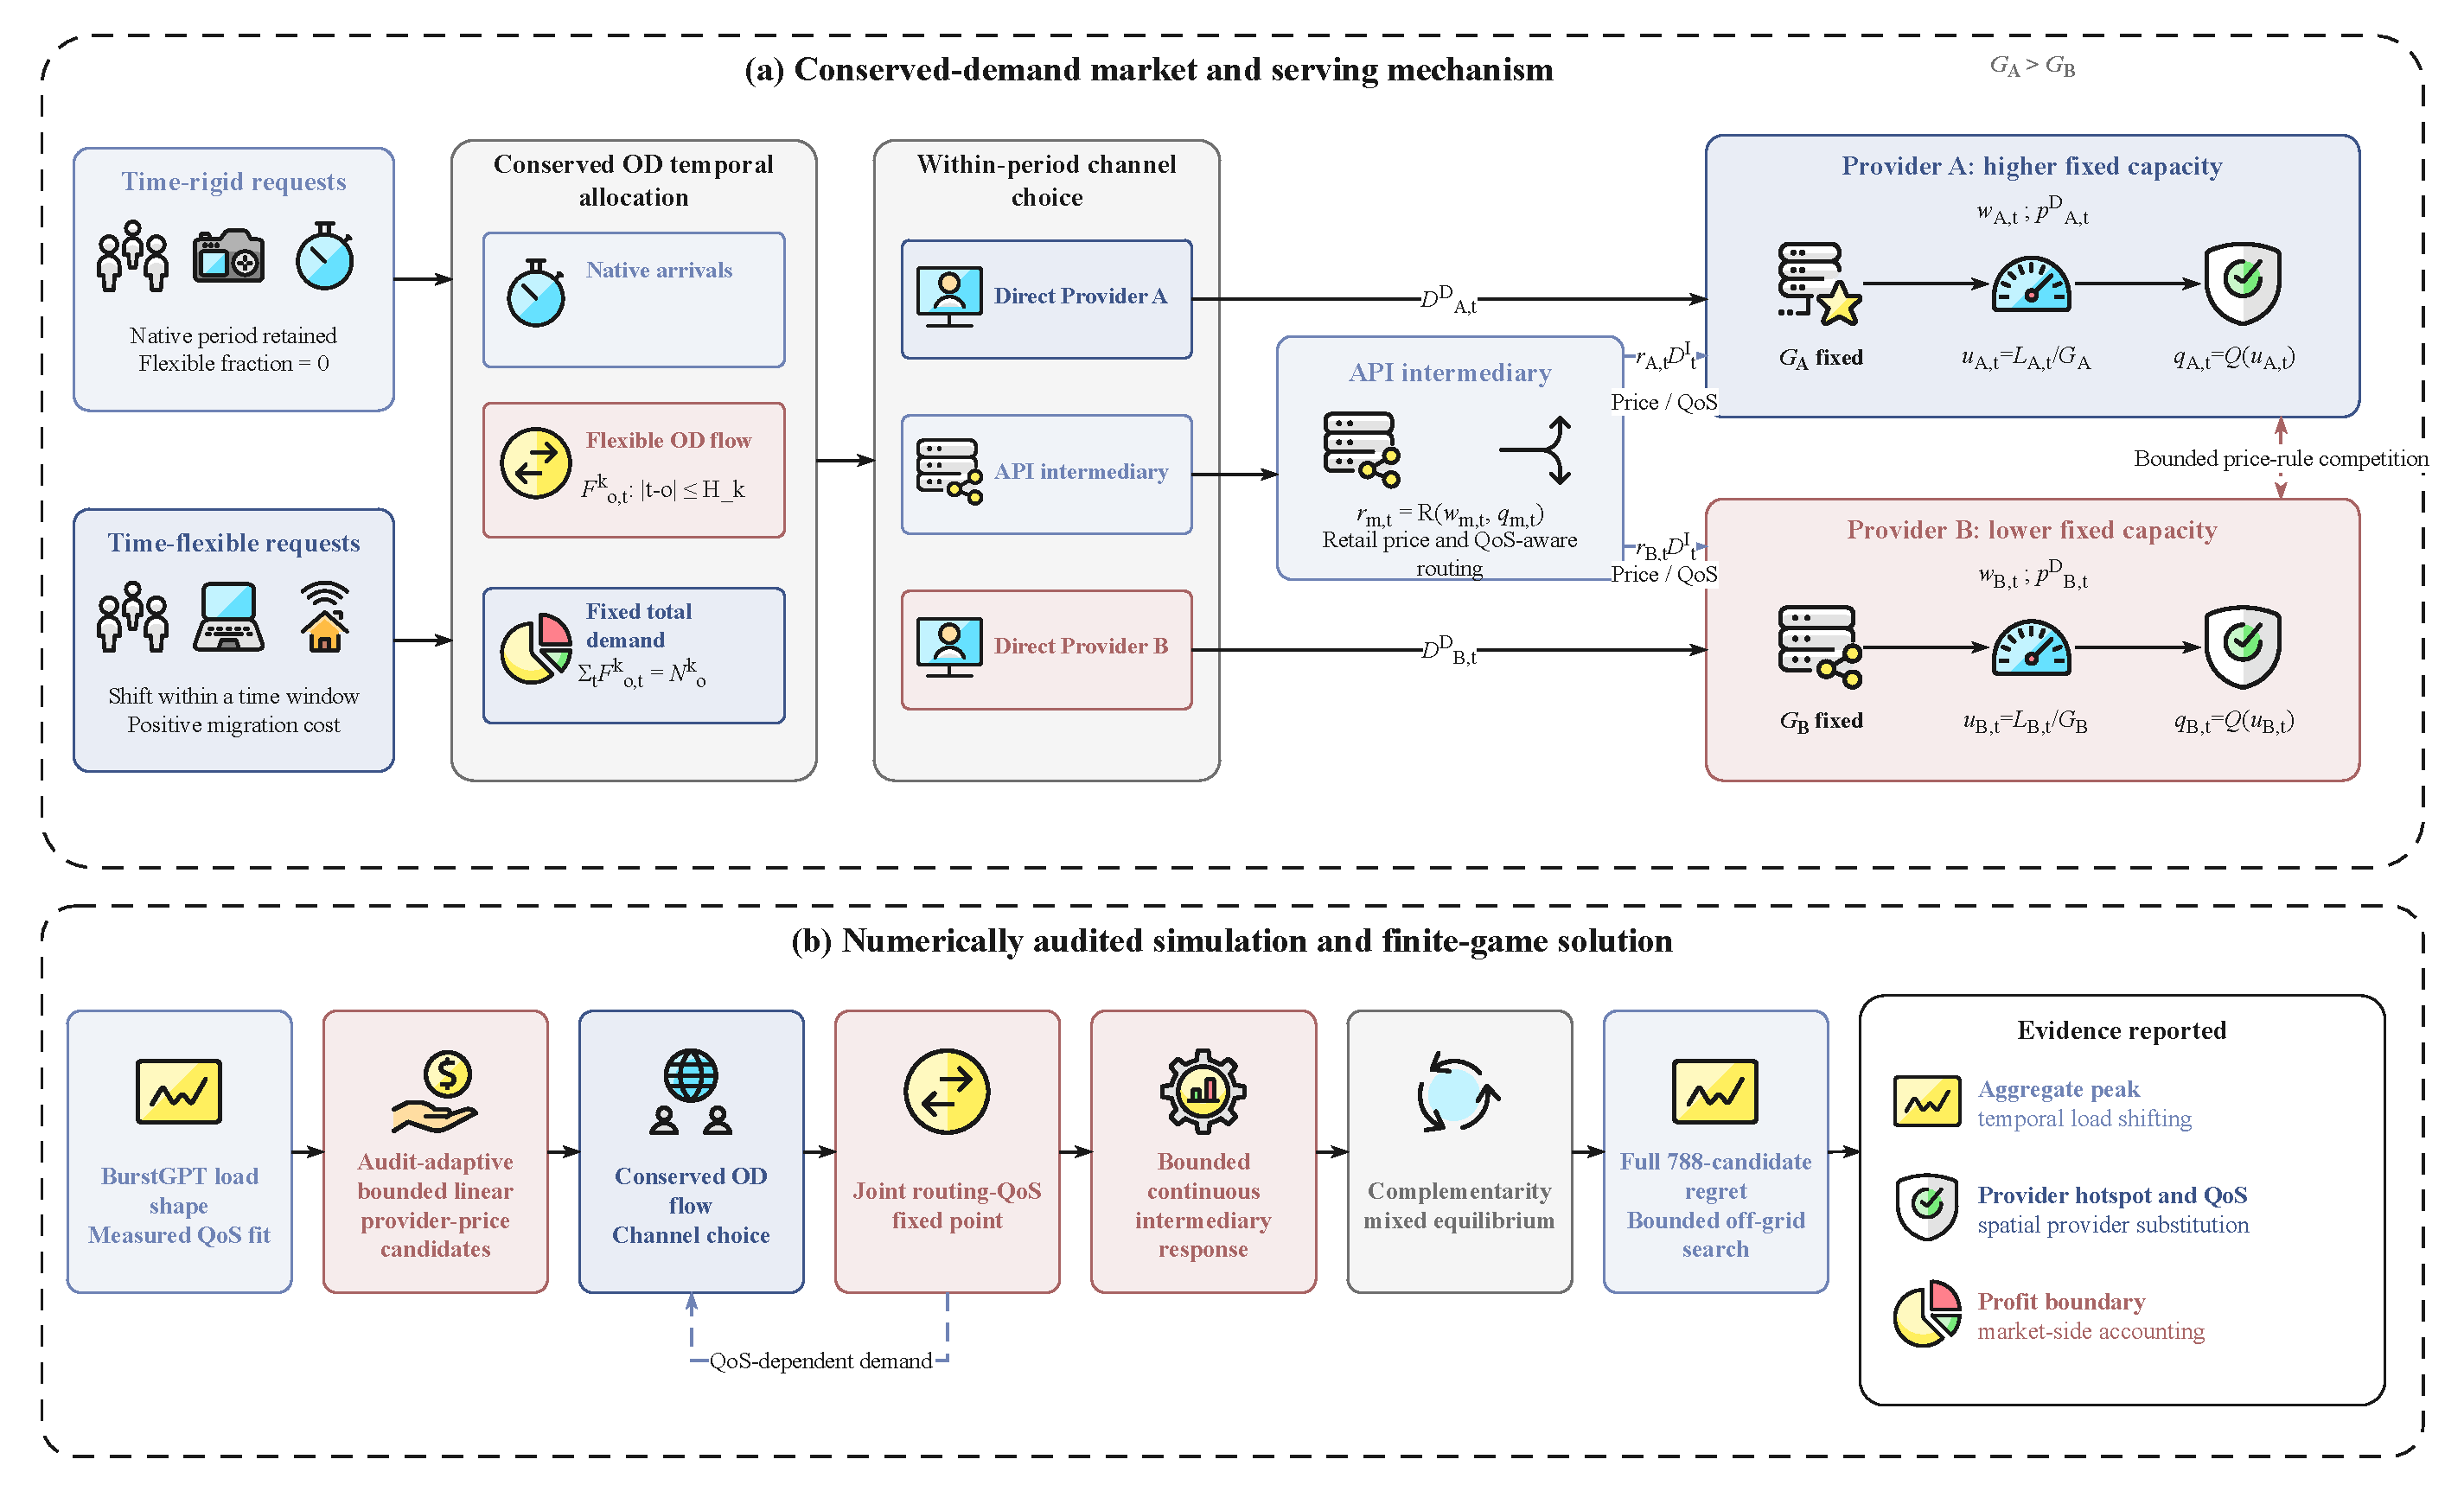
\includegraphics[width=\textwidth]{figures/peak_shaving_final_20260714/spatiotemporal_pricing_framework.pdf}
\caption{Conserved-demand market and numerical workflow. Panel (a) separates native arrivals, OD time movement, within-period channel choice, intermediary routing, and provider congestion. Solid arrows represent demand or routed traffic. Dashed arrows represent price and QoS information. Panel (b) links the two data anchors with bounded linear provider-price candidates, a bounded intermediary response, the joint market fixed point, the finite-game solution, and deviation diagnostics. Icons are from \href{https://streamlinehq.com}{Streamline Ultimate Color} under \href{https://creativecommons.org/licenses/by/4.0/}{CC BY 4.0}.}
\label{fig:framework}
\end{figure}

\subsection{Native demand and conserved temporal movement}

There are two request types, $k\in\{R,F\}$. Let $N>0$ be total native period-rate demand, $\gamma_k\ge0$ the type shares, and $\nu_o\ge0$ the normalized intraday load shares, with $\sum_k\gamma_k=\sum_o\nu_o=1$. Both types use the same observed load shape in the final design, so native demand in origin period $o$ is
\begin{equation}
N_{k,o}=N\gamma_k\nu_o.
\label{eq:native_demand}
\end{equation}
A fraction $\phi_k\in[0,1]$ may move by at most $H_k\in\mathbb Z_{\ge0}$ periods. Feasible destinations are intersected with $\T$, so the movement window does not wrap across the day boundary. The time-rigid type has $\phi_R=H_R=0$, whereas the time-flexible type has $\phi_F>0$ and $H_F>0$. The parameter $\kappa_k\ge0$ is the cost of moving one period from the origin.

The deterministic utility of channel $c$ in destination period $t$ is
\begin{equation}
V_{k,c,t}=\log b_c-\alpha_k p_{c,t}-\omega_q(1-q_{c,t}),
\label{eq:channel_utility}
\end{equation}
where $b_c>0$ is a channel preference, $\alpha_k\ge0$ is the price coefficient on utility, $\omega_q\ge0$ is the QoS weight, and $q_{c,t}$ is channel QoS. Channel prices are $p_{I,t}=p^I_t$, $p_{A,t}=p^D_{A,t}$, and $p_{B,t}=p^D_{B,t}$. Because the model has no outside option and conserves total demand, $\alpha_k$ changes allocation among period--channel alternatives; it is not an own-price elasticity of total market demand. Random utility is $U^C_{k,c,t}=V_{k,c,t}+\varepsilon^C_{k,c,t}$, where the shocks are independent type-I extreme-value variables. The resulting inclusive value of destination $t$ is
\begin{equation}
S_{k,t}=\log\left(\sum_{c\in\Channels}\exp(V_{k,c,t})\right).
\label{eq:destination_value}
\end{equation}

Destination utility is $U^T_{k,o,t}=S_{k,t}-\kappa_k|t-o|+\varepsilon^T_{k,o,t}$ inside the feasible movement window. The destination shocks are also independent type-I extreme-value variables. The scale of both shock terms is normalized to one, so $\alpha_k$ and $\kappa_k$ are interpreted relative to that utility scale. The probability of choosing period $t$ is therefore
\begin{equation}
\pi_{k,o,t}=
\begin{cases}
\displaystyle
\frac{\exp(S_{k,t}-\kappa_k|t-o|)}
{\sum_{s\in\T:\,|s-o|\le H_k}\exp(S_{k,s}-\kappa_k|s-o|)},
& t\in\T,\ |t-o|\le H_k,\\[7pt]
0, & \text{otherwise}.
\end{cases}
\label{eq:temporal_probability}
\end{equation}
The OD flow is then
\begin{equation}
F_{k,o,t}=(1-\phi_k)N_{k,o}\mathbf{1}\{t=o\}
+\phi_k N_{k,o}\pi_{k,o,t}.
\label{eq:od_flow}
\end{equation}
Equation~(\ref{eq:od_flow}) gives
\begin{equation}
\sum_{t\in\T}F_{k,o,t}=N_{k,o}
\quad\text{and}\quad
\sum_{c,t}D_{c,t}=\sum_{k,o}N_{k,o}.
\label{eq:mass_conservation}
\end{equation}
Because total demand is conserved, a lower aggregate peak cannot be produced by exit or market contraction.

\subsection{Channel choice, routing, and QoS}

After reaching destination period $t$, users choose a channel with share
\begin{equation}
s_{k,c,t}=\frac{\exp(V_{k,c,t})}{\sum_{d\in\Channels}\exp(V_{k,d,t})}.
\label{eq:channel_share}
\end{equation}
Destination demand and channel demand are
\begin{equation}
\widetilde D_{k,t}=\sum_o F_{k,o,t},
\qquad
D_{c,t}=\sum_k s_{k,c,t}\widetilde D_{k,t}.
\label{eq:channel_demand}
\end{equation}
These equations describe two stages of one conserved flow, not two sources of demand. The destination probability uses the expected value of the available channels, and the conditional channel shares then allocate that same destination demand.
The model evaluates the logit probabilities analytically and does not sample individual users or utility shocks. Conditional on a strategy profile and solver settings, the market state is deterministic. Seeds control the independent numerical audits and the vLLM measurement protocol, not simulated user draws.

The intermediary routes its demand by wholesale price and QoS:
\begin{equation}
r_{m,t}=
\frac{\exp(-\beta w_{m,t}+\eta q_{m,t})}
{\sum_{j\in\M}\exp(-\beta w_{j,t}+\eta q_{j,t})},
\qquad \sum_m r_{m,t}=1.
\label{eq:routing}
\end{equation}
Here, $\beta\ge0$ is the routing weight on wholesale price and $\eta\ge0$ is the routing weight on provider QoS. The intermediary channel QoS is $q_{I,t}=\sum_m r_{m,t}q_{m,t}$. Direct channels use the corresponding provider QoS.

Provider load and utilization are
\begin{equation}
L_{m,t}=D_{m,t}+r_{m,t}D_{I,t},
\qquad
u_{m,t}=\frac{L_{m,t}}{G_m}.
\label{eq:load_utilisation}
\end{equation}
The QoS function is the same function fitted to the vLLM measurements:
\begin{equation}
q_{m,t}=Q(u_{m,t})
=\exp\left[-\zeta\max(u_{m,t}-\bar u,0)^2\right].
\label{eq:qos}
\end{equation}
The threshold $\bar u>0$ sets the point at which degradation begins, and $\zeta>0$ controls its rate.
This reduced-form mapping permits $u_{m,t}>1$: $G_m$ is a fixed service-rate reference, and load above that reference is represented by lower QoS rather than truncated demand. The model does not simulate queue carryover between periods.

Equations~(\ref{eq:channel_utility})--(\ref{eq:qos}) form a joint fixed point in $(\boldsymbol q,\boldsymbol r)$. The implementation starts from unit QoS and equal routing, applies damping $\lambda=0.35$, and allows at most 200 iterations. The fixed-point target and damped update are
\[
\mathcal F(\boldsymbol q,\boldsymbol r)
=\bigl(Q(\boldsymbol u(\boldsymbol q,\boldsymbol r)),
R(\boldsymbol w,\boldsymbol q)\bigr),
\qquad
(\boldsymbol q^{(n+1)},\boldsymbol r^{(n+1)})
=(1-\lambda)(\boldsymbol q^{(n)},\boldsymbol r^{(n)})
+\lambda\mathcal F(\boldsymbol q^{(n)},\boldsymbol r^{(n)}).
\]
The iteration stops when
\begin{equation}
\max\left\{\|\boldsymbol q-Q(\boldsymbol u)\|_\infty,
\|\boldsymbol r-R(\boldsymbol w,\boldsymbol q)\|_\infty\right\}\le 10^{-9}.
\label{eq:joint_residual}
\end{equation}

\begin{proposition}[Existence of a market fixed point]
For fixed prices, finite native demand, and positive capacities, the market mapping has at least one fixed point in $[0,1]^{2T}\times\Delta(\M)^T$, where $\Delta(\M)=\{\boldsymbol r\in\mathbb R_+^2:r_A+r_B=1\}$.
\end{proposition}
\begin{proof}
The channel and routing shares are continuous softmax functions. The OD probabilities are continuous on their finite windows. The QoS function in Eq.~(\ref{eq:qos}) is also continuous at $u=\bar u$. Together, these functions map the compact convex set $[0,1]^{2T}\times\Delta(\M)^T$ into itself. Brouwer's fixed-point theorem guarantees at least one fixed point. This argument does not imply uniqueness or convergence of every numerical iteration.
\end{proof}

\subsection{Bounded linear price rules and accounting}

Let $\bar\nu=T^{-1}\sum_t\nu_t$ and $d_\nu=\max_s|\nu_s-\bar\nu|$. The load signal used by the price rules is
\[
\ell_t=
\begin{cases}
(\nu_t-\bar\nu)/d_\nu, & d_\nu>0,\\
0, & d_\nu=0,
\end{cases}
\qquad \ell_t\in[-1,1].
\]
Provider $m$ chooses
\begin{equation}
w_{m,t}=\operatorname{clip}\!\left(\bar w_m(1+\delta^w_m\ell_t),\underline w,\overline w\right),
\label{eq:wholesale_shape}
\end{equation}
\begin{equation}
p^D_{m,t}=\operatorname{clip}\!\left(\bar p^D_m(1+\delta^D_m\ell_t),\underline p,\overline p\right).
\label{eq:direct_shape}
\end{equation}
The intermediary uses
\begin{equation}
p^I_t=\operatorname{clip}\!\left(\bar p^I(1+\delta^I\ell_t),\underline p,\overline p\right).
\label{eq:retail_shape}
\end{equation}
Here, $\operatorname{clip}(x,a,b)=\min\{\max\{x,a\},b\}$. Each provider chooses four coefficients rather than eight wholesale and eight direct period prices. The finite candidate set discretizes these four coefficients, not the period prices: every candidate generates a bounded linear eight-period schedule through Eqs.~(\ref{eq:wholesale_shape}) and (\ref{eq:direct_shape}). The clip operator enforces posted-price bounds, so a realized schedule may be flat at a bound in some periods. These are day-ahead time-of-use schedules indexed by the fixed BurstGPT mean load signal; they do not update from realized within-day demand. The intermediary coefficients are optimized continuously within stated bounds.

Prices, capacity costs, degradation costs, and profits are expressed in normalized monetary units. They are internally comparable within the simulation but are not estimates in US dollars or any other currency.

Provider profit is
\begin{align}
\Pi_m={}&h\sum_t w_{m,t}r_{m,t}D_{I,t}q_{m,t}
+h\sum_t p^D_{m,t}D_{m,t}q_{m,t} \notag\\
&-hTc_GG_m
-hc_q\sum_t(1-q_{m,t})(D_{m,t}+r_{m,t}D_{I,t}).
\label{eq:provider_profit}
\end{align}
The intermediary profit is
\begin{align}
\Pi_I={}&h\sum_t p^I_tD_{I,t}q_{I,t}
-h\sum_{m,t}w_{m,t}r_{m,t}D_{I,t}q_{m,t} \notag\\
&-hc_q\sum_t(1-q_{I,t})D_{I,t}.
\label{eq:intermediary_profit}
\end{align}
Here, $c_G\ge0$ is the holding cost per unit of provider capacity and $c_q\ge0$ is the degradation penalty per unit of traffic. Because capacity is fixed, the capacity-cost term is constant across that provider's price strategies. It changes reported profit levels but not best-response order. For accounting, $q$ is a quality-adjusted billable fraction linked to the TTFT service-level measure. The degradation term is a separate penalty for traffic served below that level. This synthetic convention makes QoS affect both revenue and service cost. It is not an estimate of a particular API contract.

\begin{proposition}[Internal transfer conservation]
The wholesale settlement cancels exactly from aggregate market-side profit $\Pi_M=\Pi_A+\Pi_B+\Pi_I$.
\end{proposition}
\begin{proof}
For each provider and period, Eq.~(\ref{eq:provider_profit}) contains $+hw_{m,t}r_{m,t}D_{I,t}q_{m,t}$ and Eq.~(\ref{eq:intermediary_profit}) contains the same term with a negative sign. Summing the three profits removes every wholesale transfer.
\end{proof}

\subsection{Intermediary response and finite provider game}

Provider $m$ chooses the coefficient vector
\begin{equation}
\boldsymbol\theta_m=(\bar w_m,\delta^w_m,\bar p^D_m,\delta^D_m)\in\Sset.
\label{eq:provider_vector}
\end{equation}
The set $\Sset$ contains \ProviderCandidateCount{} coefficient vectors, each producing a distinct bounded price profile. Its \UniformCandidateCount{}-rule zero-slope subset combines 12 legacy anchors, a 512-point two-dimensional Latin hypercube with seed 20260716, a $9\times13$ global lattice, and two $9\times9$ local lattices. The latter three components add 114, 81, and 81 unique rules after duplicate removal. Seven additional components expand the dynamic-policy domain. An earlier candidate-expansion solve produced 52 positive-probability support entries, corresponding to 51 distinct vectors. Eighteen of those vectors were absent from the preceding union and were retained in the final set. Table~\ref{tab:candidate_design} gives the construction and cumulative counts. A vector occurring in more than one component is retained once.

\begin{table}[H]
\centering
\caption{Exact construction of the provider candidate set expanded through deviation checks. ``Added'' counts vectors not present in earlier rows; a colon denotes an inclusive equally spaced sequence.}
\label{tab:candidate_design}
\scriptsize
\begin{tabular}{@{}p{0.16\textwidth}>{\raggedright\arraybackslash}p{0.61\textwidth}rr@{}}
\toprule
Component & Coefficient values $(\bar w,\delta^w,\bar p^D,\delta^D)$ & Added & Total \\
\midrule
Uniform domain & 12 anchors; 512-point Latin hypercube; $9\times13$ global and two $9\times9$ local lattices; all slopes zero & 800 & 800 \\
Mid-slope & $\{0.25\}\times\{0.40{:}0.05{:}0.80\}\times\{0.5071875{:}0.0103125{:}0.5690625\}\times\{0.1{:}0.1{:}0.6\}$ & 378 & 1178 \\
Wholesale-base & $\bar w\in\{0.258125,0.26625\}$, $\delta^w\in\{0.45{:}0.10{:}0.85\}$; $\bar p^D\in\{0.5175,0.538125,0.55875,0.579375\}$, $\delta^D\in\{0.2,0.4,0.6\}$ & 120 & 1298 \\
Low-slope & $\bar w=0.25$, $\delta^w\in\{0,0.1,0.2,0.3\}$; $\bar p^D\in\{0.496875,0.5175,0.538125,0.55875\}$, $\delta^D\in\{0.1,0.2,0.3,0.4\}$ & 64 & 1362 \\
High-slope & $\{0.25\}\times\{1.3,1.5,1.7\}\times\{0.538125,0.55875,0.579375\}\times\{0.1,0.3,0.5\}$ & 27 & 1389 \\
Boundary guards & $\{0.25\}\times\{0.6,1,1.5,2,3\}\times\{0.45,0.60\}\times\{0,0.4,0.8,1.2,2,3\}$, union $\{0.25\}\times\{0,0.4,0.8,1.2,2,3\}\times\{0.45,0.60\}\times\{1,1.5,2,3\}$ & 100 & 1489 \\
Deviation-local & $\{0.25\}\times\{0.20,0.25,0.30\}\times\{0.5175,0.5278125,0.538125\}\times\{0.1,0.2,0.3\}$, union $\{0.25,0.258125\}\times\{0.95,1.05,1.15\}\times\{0.5175,0.5278125,0.538125\}\times\{0.3,0.4,0.5\}$ & 69 & 1558 \\
Continuation & 52 support entries, 51 distinct vectors, of which 18 are new & 18 & 1576 \\
\bottomrule
\end{tabular}
\end{table}

For completeness, the 18 continuation-only vectors are listed below in the same coefficient order as Eq.~(\ref{eq:provider_vector}):
\begin{center}
\scriptsize
\begin{tabular}{@{}lll@{}}
$(0.25,0,0.538125,0.6)$ & $(0.25,0.05,0.5175,0.2)$ & $(0.25,0.05,0.55875,0.4)$ \\
$(0.25,0.15,0.5175,0.2)$ & $(0.25,0.15,0.55875,0.4)$ & $(0.25,0.2,0.538125,0.5)$ \\
$(0.25,0.9,0.55875,0.3)$ & $(0.25,1.0,0.55875,0.3)$ & $(0.25,1.1,0.55875,0.3)$ \\
$(0.25,1.2,0.55875,0.3)$ & $(0.258125,0.3,0.538125,0.2)$ & $(0.258125,1.3,0.538125,0.3)$ \\
$(0.26625,0,0.538125,0.5)$ & $(0.26625,1.4,0.538125,0.2)$ & $(0.2825,0.9,0.55875,0.4)$ \\
$(0.29875,0.8,0.55875,0.4)$ & $(0.29875,0.9,0.55875,0.4)$ & $(0.315,0.8,0.579375,0.4)$ \\
\end{tabular}
\end{center}

For the numerical provider game, $\Pi_I(i,j,b)$ is evaluated at the market state returned by the fixed-point rule in Eq.~(\ref{eq:joint_residual}). Each evaluation starts from unit QoS and equal routing and uses the stated damping factor and tolerance. A nonconvergent evaluation is not admitted as a response candidate. For each provider pair $(i,j)$, the intermediary has the ideal target problem
\begin{equation}
b^*(i,j)\in\argmax_{b\in\mathcal B}\Pi_I(i,j,b),
\quad
\mathcal B=[0.45,2.10]\times[-1,1]\times[0,10^6],
\label{eq:intermediary_br}
\end{equation}
where $b=(\bar p^I,\delta^I,\beta)$. This continuous domain covers a declared three-parameter policy class; it does not allow unrelated retail prices or routing shares in every period. Equation~(\ref{eq:intermediary_br}) defines the ideal computational target when a maximizer is attained; no analytical existence or uniqueness result is claimed for $b^*(i,j)$. The implementation returns a numerical approximation $\widehat b(i,j)$. It uses $z=\log(1+\beta)$ to cover low and near-deterministic routing regimes and evaluates 36 deterministic coarse seeds across three routing regions. Bounded local optimization then starts from the best seed in each region. We use the limited-memory Broyden--Fletcher--Goldfarb--Shanno algorithm with box constraints (L-BFGS-B) \cite{byrd1995limited}. Each local run allows at most 250 iterations and at most 30 line-search steps per iteration. The relative objective-reduction and projected-gradient tolerances are $10^{-10}$ and $10^{-8}$. Responses within
\[
\tau_I=\max\{10^{-8},10^{-10}\max(|\Pi_I|,1)\}
\]
of the largest intermediary profit found are treated as numerical ties and resolved in favor of the smaller $\beta$. Uniform pricing fixes all provider slopes and the retail slope at zero.

The computed intermediary response induces the numerical provider payoff matrices
\begin{equation}
U^A_{ij}=\Pi_A(i,j,\widehat b(i,j)),
\qquad
U^B_{ij}=\Pi_B(i,j,\widehat b(i,j)).
\label{eq:bimatrix}
\end{equation}
Let $n_A=n_B=|\Sset|=1576$ and $\Delta_n=\{\boldsymbol z\in\mathbb R_+^n:\boldsymbol 1^\top\boldsymbol z=1\}$. The mixed strategies of the two providers are $\boldsymbol x\in\Delta_{n_A}$ and $\boldsymbol y\in\Delta_{n_B}$. A Nash equilibrium satisfies
\begin{align}
U^A\boldsymbol y&\le v_A\boldsymbol 1,
&x_i\bigl[v_A-(U^A\boldsymbol y)_i\bigr]&=0,\label{eq:nash_row_conditions}\\
\boldsymbol x^\top U^B&\le v_B\boldsymbol 1^\top,
&y_j\bigl[v_B-(\boldsymbol x^\top U^B)_j\bigr]&=0,\label{eq:nash_col_conditions}
\end{align}
with $\boldsymbol 1^\top\boldsymbol x=\boldsymbol 1^\top\boldsymbol y=1$ and non-negative probabilities. The inequalities state that no pure strategy exceeds the equilibrium payoff. Complementarity assigns positive probability only to best responses.
The scalars $v_A$ and $v_B$ are the two providers' equilibrium payoffs.
Operationally, each provider draws one complete intraday price rule before the simulated day; it does not redraw a rule in each period. The resulting distribution is a game-theoretic equilibrium object rather than a deterministic tariff recommendation.
Because each payoff entry contains a numerical intermediary response and a market fixed point, these conditions do not yield a closed-form tariff. The equilibrium of the declared finite game is therefore obtained numerically.

The numerical solver applies the following normalization separately to each provider's payoff matrix:
\begin{equation}
\widetilde U=
\begin{cases}
\displaystyle\frac{U-\min U}{\max U-\min U}, & \max U>\min U,\\[6pt]
\boldsymbol 0, & \max U=\min U.
\end{cases}
\label{eq:payoff_normalization}
\end{equation}
For a nonconstant matrix, this positive affine transformation preserves best-response order. A constant payoff matrix makes that player indifferent among its strategies. For $a,b\ge0$, define the Fischer--Burmeister function \cite{fischer1992special}
\begin{equation}
\Phi(a,b)=\sqrt{a^2+b^2}-a-b.
\label{eq:fb_function}
\end{equation}
The complementarity terms in Eqs.~(\ref{eq:nash_row_conditions}) and (\ref{eq:nash_col_conditions}) are replaced by
\begin{equation}
\Phi\!\left(x_i,v_A-(U^A\boldsymbol y)_i\right)=0,
\qquad
\Phi\!\left(y_j,v_B-(\boldsymbol x^\top U^B)_j\right)=0.
\label{eq:fb_system}
\end{equation}
Bounded nonlinear least squares solves this system, after which the probabilities are recomputed on the detected support. Each least-squares run allows 5,000 function evaluations, and the three least-squares tolerances are $10^{-13}$. Support polishing tests probability cutoffs $10^{-5},10^{-6},10^{-7},10^{-8},10^{-9}$ and retains a polished solution only when its normalized-game regret is at most $10^{-9}$. A mixed-integer complementarity formulation and bounded classical bimatrix methods are retained as fallback solvers. The final restricted equilibrium was obtained by Fischer--Burmeister support polishing. The solver does not enumerate every possible mixed equilibrium. If several numerical candidates remain, it selects the one with the lowest full-candidate regret. Restricted regret and combined provider payoff are used as tie breakers. The reported result is one verified equilibrium of the declared finite game under the evaluated numerical payoffs, not an equilibrium-selection theorem.

The restricted solution is checked against every candidate in $\Sset$. Its full-candidate regrets are
\begin{align}
\epsilon_A&=\max_i\;\boldsymbol e_i^\top U^A\boldsymbol y
-\boldsymbol x^\top U^A\boldsymbol y,\label{eq:row_regret}\\
\epsilon_B&=\max_j\;\boldsymbol x^\top U^B\boldsymbol e_j
-\boldsymbol x^\top U^B\boldsymbol y.\label{eq:col_regret}
\end{align}
Here $\boldsymbol e_i$ or $\boldsymbol e_j$ is the corresponding unit vector. The best unilateral deviations are added to the restricted game and the equilibrium is recomputed. The process stops when $\max(\epsilon_A,\epsilon_B)\le10^{-7}$. This procedure verifies the reported mixed profile against all declared candidates, not an unrestricted continuous game.

If the current row and column supports contain $s_A$ and $s_B$ strategies, a complete deviation scan evaluates at most $K(s_A+s_B)$ ordered provider pairs for $K$ candidates. Previously evaluated pairs are read from a signature-checked cache. This avoids constructing the full $K^2$ payoff matrix when the equilibrium supports remain small, although each new pair still requires an intermediary optimization and a market fixed-point solve.

The final discretization check searches the box
\begin{equation}
[0.25,0.90]\times[-4,4]\times[0.45,2.10]\times[-4,4].
\label{eq:offgrid_box}
\end{equation}
For each provider, the search combines 1,024 Latin-hypercube points \cite{mckay1979comparison} with active-support vectors and boundary guards. It also uses local one-axis perturbations and pairwise refinement around the best sampled deviation. The opponent remains at the finite-game mixed strategy. The random seed is 20260714, which differs from the seed used in the preceding candidate-expansion audit. Relative off-grid regret below 0.5\% is treated as a numerical adequacy check. It is not a proof of a continuous-space Nash equilibrium.
Let $\widehat v_m^{\mathrm{off}}$ be the largest payoff found by this search for provider $m$, and let $v_m$ be its finite-game equilibrium payoff. We report
\begin{equation}
\epsilon_m^{\mathrm{off}}=\widehat v_m^{\mathrm{off}}-v_m,
\qquad
\rho_m^{\mathrm{off}}=\epsilon_m^{\mathrm{off}}/\max\{|v_m|,1\}.
\label{eq:offgrid_regret}
\end{equation}
The 0.5\% gate applies to $\rho_m^{\mathrm{off}}$. This gate and the 0.1\% relative intermediary-profit gate used in the independent follower-response audit are prespecified numerical reporting gates, not criteria for economic significance.

\subsection{Data inputs, parameter design, and model verification}

The demand shape comes from the official BurstGPT trace \cite{wang2025burstgpt}. The pinned file contains 1,429,737 records. Requests are assigned to eight three-hour periods. The first and last partial days are removed, leaving 59 complete days. Each day is normalized to unit token mass before the period means are computed. The resulting period-share vector is
\[
\boldsymbol\nu=(0.1116,0.0273,0.0132,0.1198,0.1761,0.2169,0.1679,0.1672).
\]
Both request types use this shape, scaled by their population shares. Figure~\ref{fig:input_calibration}(a) reports the population standard deviation across the 59 retained days and uses a divisor of 59. The source does not state the time zone, so the periods describe relative positions within the recorded day rather than local clock time. The source commit, raw checksum, aggregation code, and derived profile are stored with the artifacts.

The QoS anchor uses controlled vLLM 0.22.0 measurements on one NVIDIA RTX 4090 with 24,564 MiB of memory, driver 596.21, and PyTorch 2.11.0+cu130. Both servers use automatic data type selection, a maximum model length of 2,048 tokens, and a GPU-memory-utilization setting of 0.75. The 0.5B command is stored in the benchmark run log. The 3B study artifact records the model and maximum length but not the complete command; its remaining launch flags are recovered from a contemporaneous execution log. Qwen2.5-0.5B-Instruct is tested at concurrency levels 64, 128, 224, 384, and 512 with 512 requests per level. Qwen2.5-3B-Instruct is tested at levels 32, 64, 128, 224, and 384 with 384 requests per level. The fixed prompt is ``Explain in two concise sentences why batching can improve GPU inference throughput. Do not use a list.'' Both runs use a maximum of 128 output tokens, two discarded warm-up requests, seed 42, and five repeats. Figure error bars use $t_{0.975,4}=2.776$ times the standard error across repeats. They summarize between-repeat variation, not request-level binomial uncertainty. QoS is the proportion of requests with TTFT no greater than 0.5 seconds, reported as a service-level agreement (SLA) proxy. The 0.5-second cutoff is a prespecified diagnostic threshold, not a universal production service-level objective. Concurrency divided by 224 is used as an empirical proxy for the model load ratio $u$, so $u=1$ corresponds to concurrency 224, the highest shared level with unit QoS. This proxy is not a measurement of GPU hardware utilization. The ten mean QoS points are fit by unweighted nonlinear least squares. The pooled fit constrains $\bar u\ge1$ and gives $\bar u=1.000$, $\zeta=0.5747$, and a root-mean-square error (RMSE) of $0.0561$. The threshold estimate lies on the lower fit bound. Leave-one-model-out RMSE is $0.0454$ or $0.1046$, depending on the training model.

\begin{table}[H]
\centering
\caption{Main simulation parameters and their evidence status.}
\label{tab:parameters}
\small
\begin{tabular}{@{}lll@{}}
\toprule
Parameter & Main value & Basis \\
\midrule
Periods and period length & $T=8$, $h=3$ hours & BurstGPT aggregation \\
Sum of native period rates & 1100 normalized units & Fixed simulation scale \\
Rigid/flexible population share & $0.4/0.6$ & Synthetic design \\
Reallocatable fraction $\phi_R/\phi_F$ & $0/0.8$ & Synthetic design \\
Utility price coefficient $\alpha_R/\alpha_F$ & $2/5$ & Synthetic design \\
Migration cost $\kappa_R/\kappa_F$ & $2/0.35$ & Synthetic; inactive for $R$ \\
Maximum shift $H_R/H_F$ & $0/2$ periods & Synthetic design \\
Provider capacities $G_A/G_B$ & $180/72$ rate units & Congested stress case \\
QoS threshold and strength & $1.000/0.5747$ & Pooled vLLM fit \\
QoS choice weight $\omega_q$ & 1 & Synthetic design \\
Routing QoS weight $\eta$ & 3 & Synthetic design \\
Channel preferences $(b_I,b_A,b_B)$ & $(1.05,1,1)$ & Synthetic design \\
Fixed shares when spatial response is off & $(0.12,0.50,0.38)$ & Decomposition control \\
Capacity/degradation cost & $0.015/0.35$ & Synthetic design \\
Wholesale/direct posted-price bounds & $[0.25,0.90]/[0.45,2.10]$ & Numerical design \\
Intermediary $(\bar p^I,\delta^I,\beta)$ bounds & $[0.45,2.10]/[-1,1]/[0,10^6]$ & Numerical search design \\
\bottomrule
\end{tabular}
\end{table}

Table~\ref{tab:parameters} lists the main parameter values and distinguishes external anchors from synthetic design choices. The capacity pair $(180,72)$ creates an asymmetric congestion stress case in normalized service-rate units. It is not converted from the RTX 4090 measurements and does not represent a count of physical GPUs. Model verification is separate from empirical input anchoring. Automated tests verify OD row conservation, total demand, wholesale transfer cancellation, price-shape signs, fixed-point residuals, finite-game regret, deterministic artifacts, and figure inputs. Within an intermediary search, a response evaluation is discarded if its joint fixed point does not converge. Empirical anchoring is limited to the mean BurstGPT load shape and the measured single-GPU QoS shape. The simulated market outcomes are not externally validated. Utility price coefficients, migration cost, capacity, and cost parameters remain synthetic.

For a mixed provider profile $(I,J)\sim\boldsymbol x\times\boldsymbol y$, the reported expectation of a profile statistic $g$ is
\begin{equation}
\mathbb E[g]=\sum_i\sum_j x_i y_j g_{ij}.
\label{eq:mixed_expectation}
\end{equation}
The main congestion and QoS measures are
\begin{align}
L_{\mathrm{peak}}&=\mathbb E\!\left[\max_t\sum_m L_{m,t}\right],
&u_{\max}&=\mathbb E\!\left[\max_{m,t}u_{m,t}\right],\label{eq:peak_metrics}\\
q_{\min}&=\mathbb E\!\left[\min_{m,t}q_{m,t}\right],
&\overline{\Pi}_M&=\mathbb E[\Pi_A+\Pi_B+\Pi_I].\label{eq:qos_profit_metrics}
\end{align}
Because $N$ is conserved in every profile, the reported peak-to-average ratio and temporally moved fraction are
\begin{equation}
R_P=L_{\mathrm{peak}}/(N/T),
\qquad
M=\mathbb E\!\left[\frac{\sum_{k,o}\sum_{t\ne o}F_{k,o,t}}{N}\right].
\label{eq:movement_metrics}
\end{equation}
The destination-period centroid for request type $k$ is
\begin{equation}
C_k=
\frac{\sum_{t=1}^{T}t\,\mathbb E[\widetilde D_{k,t}]}
{\sum_{t=1}^{T}\mathbb E[\widetilde D_{k,t}]}.
\label{eq:destination_centroid}
\end{equation}
Here the period indices are one based, so a lower value denotes an earlier average destination period.
Tables report these profile-level expectations. Profile figures instead show period-by-period expectations. In general, $\mathbb E[\max X]\ne\max\mathbb E[X]$ and $\mathbb E[\min X]\ne\min\mathbb E[X]$.

A fixed-profile decomposition separates the intraday shape of the dynamic prices from changes in their average levels and equilibrium mixture. For every active dynamic provider pair, each realized wholesale, direct, and intermediary retail schedule is replaced by its own period mean. The routing parameter and equilibrium pair weights are held fixed, and the market fixed point is re-solved. This removes within-day price variation while preserving the average of every realized price series. If $g_U$, $g_D$, and $g_F$ denote the equilibrium under the uniform-price restriction, the time-varying equilibrium, and the mean-flattened dynamic-profile value of metric $g$, then
\begin{equation}
g_D-g_U=(g_D-g_F)+(g_F-g_U).
\label{eq:price_shape_decomposition}
\end{equation}
The first term is the fixed-profile shape component. The second contains price-level and equilibrium-composition differences. This accounting identity does not re-optimize any player's strategy.

The sensitivity study re-solves the uniform and dynamic games for the baseline and eight local, one-factor-at-a-time perturbations. Both provider capacities are jointly scaled by 0.85 or 1.15, which preserves the baseline ratio $G_A/G_B=2.5$. Both type-specific utility price coefficients are jointly scaled by 0.8 or 1.2, preserving $\alpha_F/\alpha_R=2.5$. Both migration-cost entries are jointly scaled by 0.7 or 1.3. Because $\phi_R=H_R=0$, this last perturbation changes only the flexible type's temporal allocation in the computed flows. The QoS threshold is shifted by $-0.05$ or $+0.05$. Thus, the study changes parameter levels while keeping the main capacity and behavioral heterogeneity ratios fixed; it does not estimate interactions among parameters. Every case uses the common 1,576-candidate provider set and the bounded continuous intermediary response. The uniform restriction uses the full 800-rule zero-slope subset. Each case re-solves the finite game and checks every declared unilateral provider deviation against the resulting support. It need not construct all $1576^2$ payoff cells. A nine-scenario uniform-price off-grid audit evaluates the two-dimensional zero-slope domain, while the baseline four-dimensional off-grid audit checks the richer dynamic-policy domain.

\section{Experimental results}
\label{sec:results}

\subsection{Load and QoS inputs}

Figure~\ref{fig:input_calibration} reports the two external anchors. BurstGPT token demand is lowest in periods 2 and 3 and highest in period 6. The between-day standard deviations are large, so the trace is used only for the mean daily shape. The vLLM points remain at unit SLA rate up to a normalized concurrency of one and decline at higher concurrency. The pooled curve reproduces this threshold pattern and serves as a controlled QoS-shape input, not as a production-cluster model.

\begin{figure}[H]
\centering
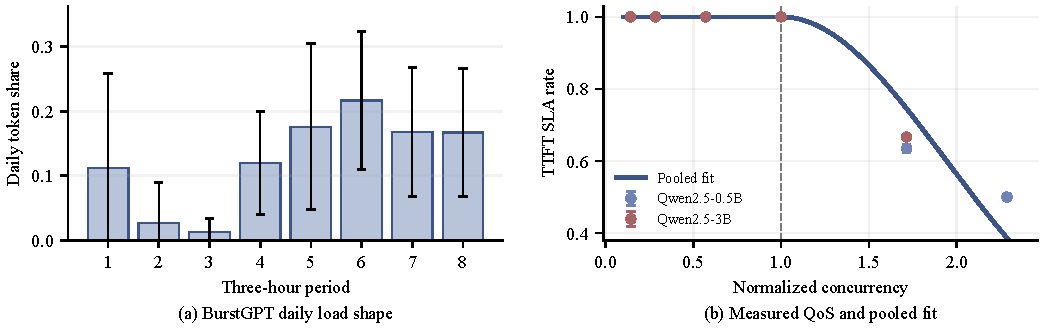
\includegraphics[width=\textwidth]{figures/peak_shaving_final_20260714/input_calibration.pdf}
\caption{Inputs used to anchor the final simulation. Panel (a) shows the mean and standard deviation of day-normalized BurstGPT token shares across 59 complete days. Panel (b) shows mean controlled vLLM TTFT-SLA measurements across five repeats, repeat-level Student-$t$ 95\% confidence intervals, and the pooled threshold-exponential fit.}
\label{fig:input_calibration}
\end{figure}

\subsection{Finite-game equilibria and main comparison}

The main comparison changes the allowed policy class for the whole market. The restricted game fixes all provider slopes and the intermediary retail slope at zero, whereas the time-varying game permits both. It is not an experiment that changes one posted price while holding every other decision fixed; it compares two internally solved market regimes.

The numerical uniform-price payoff matrix has a mixed equilibrium over ten positive-probability strategies for each provider. Their probability-weighted coefficient means are $(0.3537,0,0.5912,0)$ and $(0.2941,0,0.6020,0)$ for providers A and B. The time-varying payoff matrix also has a mixed equilibrium and assigns positive probability to 26 strategies for each provider. All reported mixtures are verified against every rule in their respective 800- and 1,576-candidate games.

Provider A's active wholesale slopes range from 0 to 1.2, and provider B's range from 0 to 1.5. Their probability-weighted coefficient means are $(0.2708,0.6401,0.5492,0.3028)$ and $(0.2520,0.4344,0.5368,0.4796)$, respectively. These means summarize the mixed strategy; they should not be read as a separate equilibrium action.

The intermediary response also varies across the active provider pairs. The lower bound $\beta=0$ carries 29.0\% of the profile probability mass, while the upper bound near $10^6$ carries only 0.013\%. At least one period has near-deterministic routing in profiles with 24.9\% probability mass. These boundary and concentration patterns motivate treating $\beta$ as a numerical routing control rather than an estimated economic elasticity.

\begin{table}[H]
\centering
\caption{Uniform and time-varying finite-game outcomes. Peak, utilization, and QoS entries are expectations of the profile-level extrema defined in Eqs.~(\ref{eq:peak_metrics}) and (\ref{eq:qos_profit_metrics}). Profit entries use normalized monetary units.}
\label{tab:main_results}
\small
\begin{tabular}{@{}lrrr@{}}
\toprule
Metric & Uniform & Time-varying & Change \\
\midrule
Aggregate peak load & \UniformAggregatePeak{} & \DynamicAggregatePeak{} & $\AggregatePeakChangePercent\%$ \\
Aggregate peak-to-average ratio & \UniformPeakToAverage{} & \DynamicPeakToAverage{} & $\AggregatePeakChangePercent\%$ \\
Maximum provider utilization & \UniformMaximumUtilisation{} & \DynamicMaximumUtilisation{} & $\MaximumUtilisationChangePercent\%$ \\
Minimum provider QoS & \UniformMinimumQoS{} & \DynamicMinimumQoS{} & $+\MinimumQoSChange$ \\
Temporally moved fraction & \UniformMovedFraction{} & \DynamicMovedFraction{} & $+\MovedFractionChange$ \\
Provider $A$ profit & \UniformProviderAProfit{} & \DynamicProviderAProfit{} & $\ProviderAProfitChangePercent\%$ \\
Provider $B$ profit & \UniformProviderBProfit{} & \DynamicProviderBProfit{} & $+\ProviderBProfitChangePercent\%$ \\
Intermediary profit & \UniformIntermediaryProfit{} & \DynamicIntermediaryProfit{} & $+\IntermediaryProfitChangePercent\%$ \\
Aggregate market-side profit & \UniformMarketProfit{} & \DynamicMarketProfit{} & $+\MarketProfitChangePercent\%$ \\
\bottomrule
\end{tabular}
\end{table}

Table~\ref{tab:main_results} shows a 28.141-unit reduction in the expected profile peak. The largest period-level reduction occurs in period 6. The uniform aggregate peak, \UniformAggregatePeak{}, is below the combined provider capacity of 252, but provider B reaches an expected utilization of 1.369 in period 6. Congestion is therefore a provider-level hotspot caused by heterogeneous capacities and traffic allocation, rather than a market-wide capacity shortfall. Provider B remains the tighter-capacity provider. Its highest expected utilization moves from period 6 to period 7 and falls from 1.369 to 1.202. The minimum of the expected QoS curves rises from 0.9012 to \DynamicMinimumQoS{}. The profile-level statistic in Table~\ref{tab:main_results} is $\mathbb E[\min_{m,t}q_{m,t}]=\DynamicMinimumQoS$; the values differ before rounding. The expected profile-level maximum utilization remains above one at \DynamicMaximumUtilisation{}, so the time-varying equilibrium reduces rather than eliminates modeled overload.

The realized end-user price profiles are shown in Fig.~\ref{fig:equilibrium_profiles}(b). Probability-weighted intermediary and direct prices are lowest in periods 2--3 and highest in period 6. They remain below their uniform-price counterparts in every period. The uniform result is the equilibrium under the uniform-price restriction, so it need not remain stable when sloped price rules are admitted. Since demand is conserved and there is no outside option, temporal movement is driven by relative prices within each schedule rather than by a change in market size.

Because the time-varying outcome is mixed, its profile distribution is also relevant. Table~\ref{tab:mixed_distribution} reports weighted quantiles across the 676 positive-probability provider pairs. Each quantile is the smallest observed profile value whose cumulative probability reaches the stated level. These quantiles describe equilibrium randomization and are not confidence intervals. The lowest QoS observed across the active pairs is 0.893, below the uniform equilibrium expectation \UniformMinimumQoS{} but above the lowest period-level dynamic expected QoS.

\begin{table}[H]
\centering
\caption{Outcome distribution across active time-varying provider pairs. Profit uses normalized monetary units.}
\label{tab:mixed_distribution}
\small
\begin{tabular}{@{}lrrr@{}}
\toprule
Metric & 5th percentile & Median & 95th percentile \\
\midrule
Aggregate peak load & 194.639 & 195.162 & 202.729 \\
Maximum provider utilization & 0.933 & 1.289 & 1.390 \\
Minimum provider QoS & 0.916 & 0.953 & 1.000 \\
Aggregate market-side profit & 1849.373 & 1934.681 & 1979.354 \\
\bottomrule
\end{tabular}
\end{table}

\begin{figure}[H]
\centering
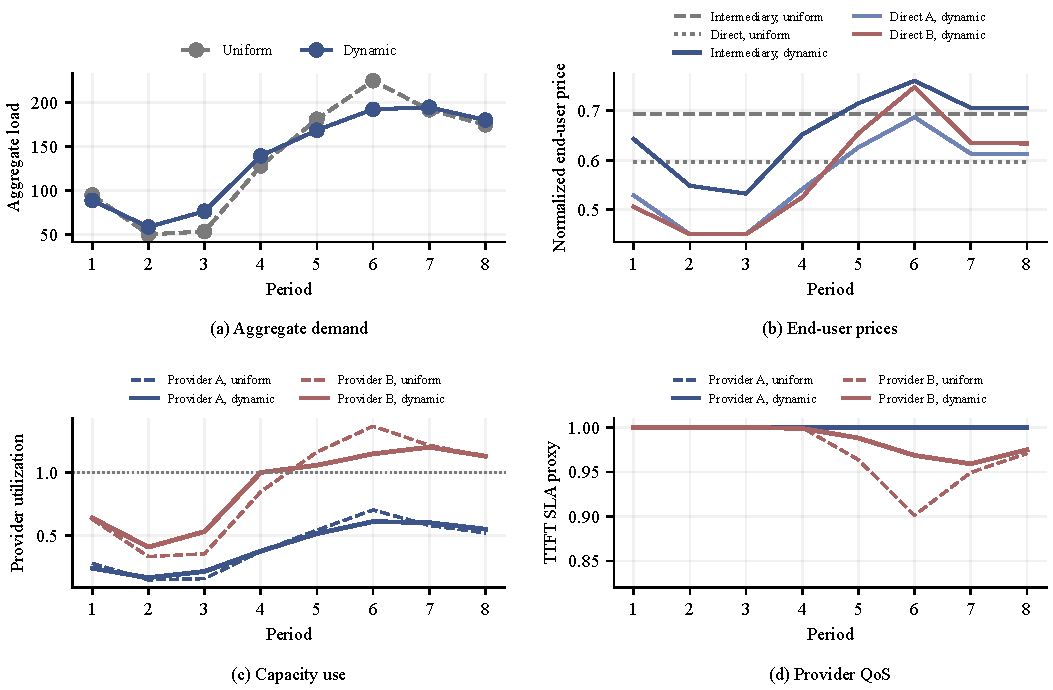
\includegraphics[width=\textwidth]{figures/peak_shaving_final_20260714/equilibrium_profiles.pdf}
\caption{Period-level expected profiles under uniform and time-varying pricing. Panel (a) reports aggregate load, panel (b) end-user prices, panel (c) provider utilization, and panel (d) the TTFT-SLA proxy. Direct prices for the two providers coincide under uniform pricing. The highest expected time-varying load is 194.865, whereas Table~\ref{tab:main_results} reports $\mathbb E[\max_t L_t]=196.903$. The same distinction applies to utilization and QoS.}
\label{fig:equilibrium_profiles}
\end{figure}

The demand result is not caused by market exit. The sum of normalized period-rate demand is 1100 under both equilibria by construction and by artifact check. The flexible-demand centroid changes from 5.304 to 5.200. The full OD matrix gives a temporally moved fraction of 0.327 under time-varying pricing, compared with 0.313 under uniform pricing. The 1.38-percentage-point increase is small relative to the peak reduction, so the destination pattern matters more than the total amount moved.

\subsection{Numerical equilibrium checks}

The augmented reconstruction uses 43,246 distinct provider pairs for the 800-rule uniform game and 81,276 pairs for the 1,576-rule dynamic game. The uniform double oracle reaches a full-candidate regret of $2.27\times10^{-13}$ after 30 support-expansion rounds. The dynamic continuation support passes its full-grid scan at $1.14\times10^{-13}$ in the first augmented reconstruction round. The largest joint routing--QoS residual is below $1.0\times10^{-9}$ in both games.

Both pair sets were loaded from signature-checked persistent caches during the formal reconstruction, and no additional follower evaluations were required in that reconstruction command. These sparse sets are numerical-oracle caches rather than complete $800^2$ or $1576^2$ payoff matrices. The runtime of the preceding cache construction is therefore not presented as a from-scratch benchmark.

An independent differential-evolution search \cite{storn1997differential} re-optimized the intermediary response for all 676 positive-probability provider pairs. The base seed was 20260713, with the profile index added for each run. It used 35 generations, a population multiplier of 8, and absolute and relative tolerances of $10^{-8}$ before local polishing. The largest profit improvement was 0.1027, or 0.0292\% relative to the stored intermediary profit, below the declared 0.1\% audit threshold. The largest joint fixed-point residual was $1.0\times10^{-9}$. The $1.14\times10^{-13}$ provider regret applies to the declared finite provider game under the cached payoff evaluations. Practical numerical accuracy also depends on the follower-response audit. Of the 676 runs, 381 met the optimizer's stopping criterion. The other 295 reached the iteration limit, but none improved the stored response by more than $3.16\times10^{-10}$ in relative terms. This is a full-active-profile numerical check, not a proof of global optimality.

Initial-condition sensitivity was checked separately. Each active provider pair was solved from 32 random QoS and routing states. The base seed was 20260713, with the profile index added before its initial states were generated. All 21,632 runs converged. The largest residual was $1.00\times10^{-9}$, while the largest endpoint spans were $9.70\times10^{-10}$ for QoS and $2.07\times10^{-9}$ for routing. No multiple fixed points were observed in this audit, although the result is not an analytical uniqueness proof.

Dependence on the mixed-equilibrium starting point was also checked on the frozen $26\times26$ restricted payoff matrices. The reported solution, a uniform start, and 64 independently generated Dirichlet starts were used. The Dirichlet generator used seed 20260715. All 66 starts returned a valid equilibrium. All valid solutions belonged to the same numerical branch at a probability tolerance of $10^{-6}$ and reproduced the 26-by-26 active support. The branch retained full-candidate regret of $3.41\times10^{-13}$ and the same four main outcome metrics to floating-point precision. This multistart result checks recovery of the reported branch but does not enumerate or prove uniqueness of every bimatrix equilibrium.

The independent bounded search evaluated 1,720 deviations for provider A and 1,699 for provider B. It included the active support, 1,024 Latin-hypercube points, boundary guards, local perturbations, and pairwise refinement. The best relative off-grid regrets were 0.400\% for A and 0.473\% for B. Both are below the declared 0.5\% numerical-adequacy threshold, while remaining nonzero numerical gaps. The best omitted vectors were $(0.25,0.35,0.538125,0.2)$ for A and $(0.2825,-0.15,0.5278125,0.5)$ for B. Every evaluated joint fixed point converged, the largest residual was $1.00\times10^{-9}$, and the largest active-support payoff error was $6.82\times10^{-13}$. Figure~\ref{fig:solver_diagnostics} places these checks beside the finite-game convergence and follower audits. The result supports the declared finite grid and its local neighborhood; it does not establish a continuous-strategy equilibrium.

\begin{figure}[H]
\centering
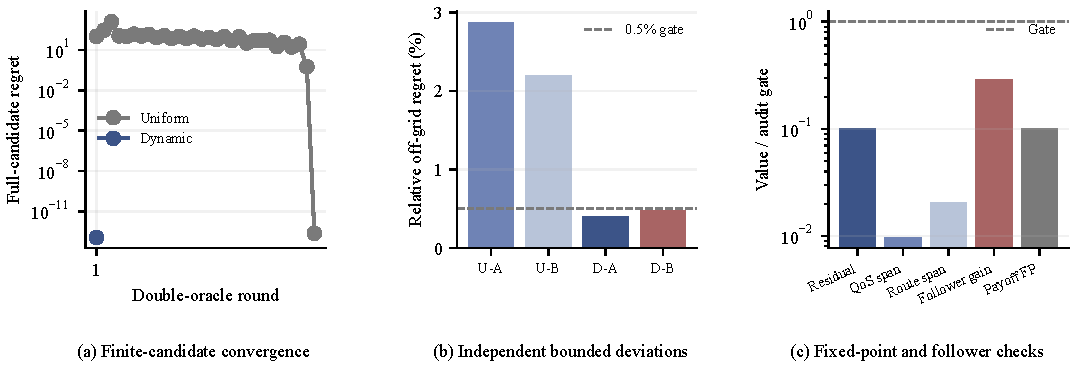
\includegraphics[width=\textwidth]{figures/peak_shaving_final_20260714/solver_diagnostics.pdf}
\caption{Numerical equilibrium checks. Panel (a) reports full-candidate regret over double-oracle rounds. Panel (b) reports relative regret from the independent bounded off-grid search; the dashed line is the declared 0.5\% adequacy threshold. Panel (c) scales the fixed-point residual, endpoint spans, and intermediary profit improvement by their respective audit thresholds; values below one pass the stated checks.}
\label{fig:solver_diagnostics}
\end{figure}

\subsection{Temporal and spatial mechanism decomposition}

The main comparison contains both time movement and spatial substitution. The final decomposition fixes each active profile's provider and intermediary price decisions, then re-solves demand and QoS with temporal response, spatial response, both responses, or neither response. When spatial response is disabled, user channel shares are held at $(0.12,0.50,0.38)$ and intermediary traffic is split between the providers in proportion to their fixed capacities. Temporal choice then uses the fixed-share-weighted mean of the three channel utilities as its destination value. When spatial response is enabled, channel choice and intermediary routing respond to prices and QoS, and temporal choice uses the log-sum inclusive value in Eq.~(\ref{eq:destination_value}). Profile results are averaged with the equilibrium probabilities. This is a fixed-policy decomposition and not a new equilibrium for each mechanism switch.

Compared with uniform pricing under the same response setting, the temporal-only case reduces aggregate peak and maximum provider utilization by 13.03\% and raises minimum QoS by 0.0408. The spatial-only case leaves aggregate peak unchanged, because requests do not move across periods, but lowers maximum provider utilization by 4.32\% and raises minimum QoS by 0.0265. With both responses enabled, the augmented-baseline changes are $\AggregatePeakChangePercent$\%, $\MaximumUtilisationChangePercent$\%, and $+\MinimumQoSChange$, respectively. Figure~\ref{fig:mechanism_decomposition} summarizes these fixed-policy differences. The three comparisons are not additive because channel choice, routing, and QoS are re-solved together in each setting. Their isolated values also depend on the fixed channel shares and capacity-proportional routing used as the spatial-off reference.

Spatial response is not uniformly beneficial relative to a capacity-proportional fixed route. Within the time-varying equilibrium, enabling spatial choice raises maximum utilization from 1.131 in the temporal-only control to \DynamicMaximumUtilisation{}. Minimum QoS falls from 0.990 to \DynamicMinimumQoS{}. The intermediary sends 57.1\% of its traffic to provider A in the combined case, below A's 71.4\% share of total capacity. The combined equilibrium improves utilization and QoS relative to the equilibrium under the uniform-price restriction, but its endogenous route still places disproportionate load on the smaller provider.

\begin{figure}[H]
\centering
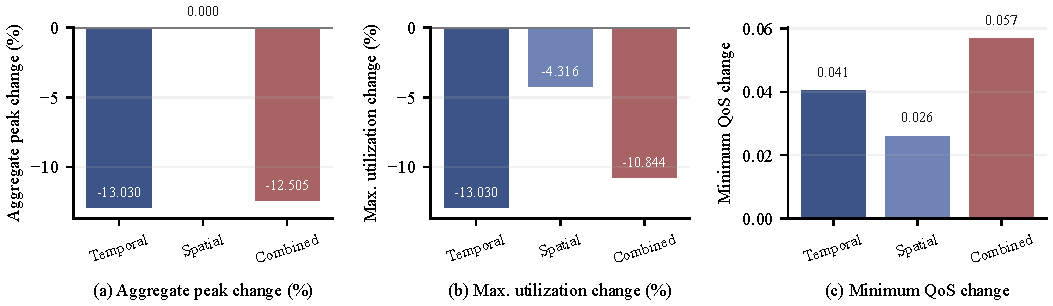
\includegraphics[width=\textwidth]{figures/peak_shaving_final_20260714/mechanism_decomposition.pdf}
\caption{Fixed-policy mechanism comparisons. Each bar is the time-varying result minus the uniform-price result under the same response setting. Panel (a) shows aggregate peak change, panel (b) maximum provider-utilization change, and panel (c) minimum-QoS change. Spatial response alone cannot change the aggregate period load because total demand is conserved and temporal movement is disabled. The three response settings are re-solved separately and are not additive.}
\label{fig:mechanism_decomposition}
\end{figure}

The price-shape decomposition gives a separate check on interpretation. Mean-flattening the dynamic profiles raises aggregate peak load from \DynamicAggregatePeak{} to 225.434 and maximum provider utilization from \DynamicMaximumUtilisation{} to 1.354. Minimum QoS falls from \DynamicMinimumQoS{} to 0.918. Table~\ref{tab:price_shape_decomposition} separates the intraday shape from the price-level and equilibrium-composition remainder; its values are regenerated from the augmented baseline before the final evidence gate.

\begin{table}[H]
\centering
\caption{Fixed-profile price-shape decomposition. Overall change equals the shape component plus the price-level and equilibrium-composition remainder. Profit is in normalized monetary units.}
\label{tab:price_shape_decomposition}
\small
\begin{tabular}{@{}lrrr@{}}
\toprule
Metric & Overall change & Shape component & Level/mix remainder \\
\midrule
Aggregate peak load & $-28.141$ & $-28.531$ & $+0.390$ \\
Maximum provider utilization & $-0.1487$ & $-0.1312$ & $-0.0175$ \\
Minimum provider QoS & $+0.0574$ & $+0.0408$ & $+0.0166$ \\
Aggregate market-side profit & $+42.000$ & $+107.502$ & $-65.502$ \\
\bottomrule
\end{tabular}
\end{table}

The profit decomposition differs from the congestion results. Restoring the dynamic price shapes to the mean-flattened profiles raises aggregate market-side profit by 107.502, while the level-and-mix remainder is $-65.502$. The net result is the 42.000-unit increase in Table~\ref{tab:main_results}. This fixed-profile comparison helps locate the difference; it is not a claim that either component is an equilibrium payoff effect in isolation.

\subsection{Sensitivity analysis}

The final sensitivity study uses the common 1,576-candidate set and re-solves the two provider games with the continuous intermediary response. It covers the baseline and eight local perturbations defined in Section~\ref{sec:methodology}. The analysis reports finite-candidate regret, fixed-point residuals, congestion measures, QoS, and aggregate market-side profit for every case.

Table~\ref{tab:resolved_sensitivity} gives the audited scenario-level results. Across the declared local perturbations, peak load and maximum utilization fall and minimum QoS rises relative to the corresponding equilibrium under the uniform-price restriction. Aggregate market-side profit is not sign-robust across the sensitivity cases, so it is reported as an accounting outcome rather than a welfare conclusion.

% Generated from the audited sensitivity summary. Do not edit.
% Source SHA-256: 7bfbd0d471a73ffe23b50034c463b536c9ea0e601a86e7c6f59f8d8bbaa41626
\begin{table}[H]
\centering
\caption{Finite-game sensitivity results on the common 1,576-candidate set. Each case re-solves both policy games and checks every declared unilateral provider deviation. Maximum regret is the larger uniform or time-varying finite-game value. Maximum residual is taken across both games. Peak, utilization, and profit changes are percentages; minimum-QoS change is absolute.}
\label{tab:resolved_sensitivity}
\scriptsize
\setlength{\tabcolsep}{2.25pt}
\begin{tabular}{@{}lrrrrrr@{}}
\toprule
Case & Maximum regret & Maximum residual & Peak $\Delta$ (\%) & Utilization $\Delta$ (\%) & Minimum QoS $\Delta$ & Profit $\Delta$ (\%) \\
\midrule
Baseline & $2.27\times10^{-13}$ & $1.00\times10^{-9}$ & $-12.50$ & $-10.84$ & $+0.0574$ & $+2.23$ \\
Capacity $-15\%$ & $3.41\times10^{-13}$ & $9.99\times10^{-10}$ & $-13.36$ & $-10.91$ & $+0.0662$ & $-9.14$ \\
Capacity $+15\%$ & $2.27\times10^{-13}$ & $9.95\times10^{-10}$ & $-12.98$ & $-7.62$ & $+0.0279$ & $+0.49$ \\
Utility coefficient $-20\%$ & $3.38\times10^{-11}$ & $1.00\times10^{-9}$ & $-12.84$ & $-8.80$ & $+0.0423$ & $-9.49$ \\
Utility coefficient $+20\%$ & $2.27\times10^{-13}$ & $1.00\times10^{-9}$ & $-11.98$ & $-10.38$ & $+0.0533$ & $+0.01$ \\
Migration cost $-30\%$ & $2.27\times10^{-13}$ & $9.99\times10^{-10}$ & $-13.08$ & $-11.52$ & $+0.0603$ & $+1.92$ \\
Migration cost $+30\%$ & $2.27\times10^{-13}$ & $1.00\times10^{-9}$ & $-12.00$ & $-10.59$ & $+0.0553$ & $+2.14$ \\
QoS threshold $-0.05$ & $3.41\times10^{-13}$ & $9.98\times10^{-10}$ & $-12.35$ & $-10.90$ & $+0.0534$ & $-0.32$ \\
QoS threshold $+0.05$ & $6.82\times10^{-13}$ & $1.00\times10^{-9}$ & $-12.78$ & $-11.19$ & $+0.0583$ & $+1.46$ \\
\bottomrule
\end{tabular}
\end{table}


Figure~\ref{fig:resolved_sensitivity} summarizes the same sensitivity evidence as signed changes in congestion, service quality, and aggregate market-side profit. The plotted factors are local level changes around the synthetic calibration, not an interaction design or a production uncertainty distribution.

\begin{figure}[H]
\centering
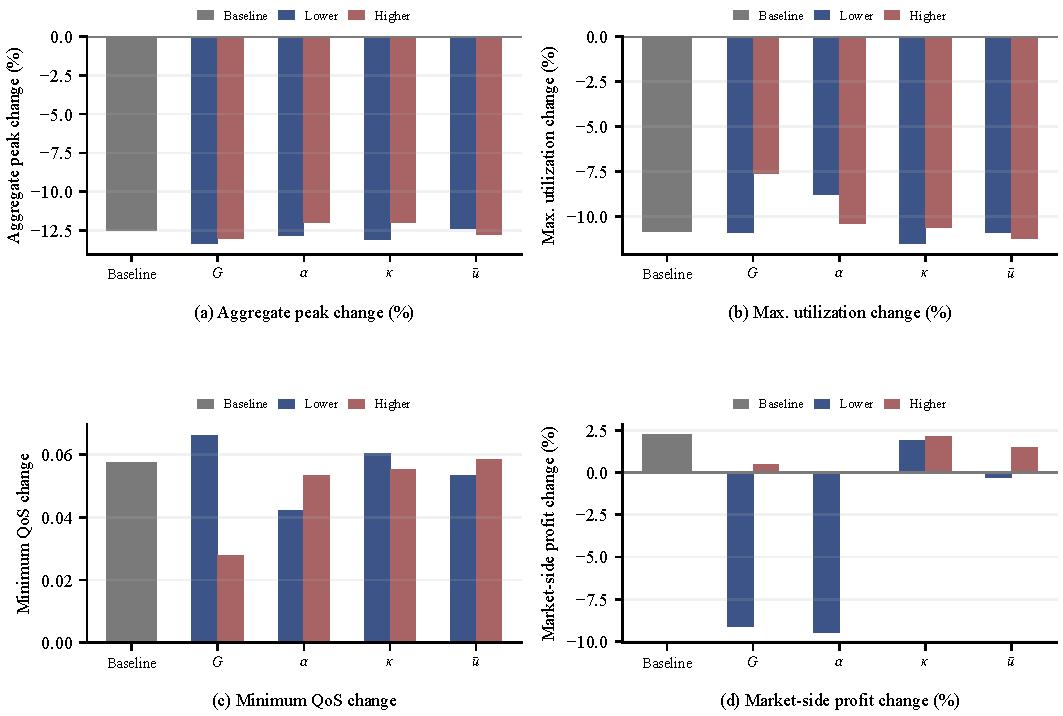
\includegraphics[width=\textwidth]{figures/peak_shaving_final_20260714/resolved_sensitivity.pdf}
\caption{Resolved finite-game sensitivity cases. Each panel uses the common 1,576-candidate provider set and the continuous intermediary response. The baseline row is included as the reference scenario; lower and higher perturbations are paired by factor.}
\label{fig:resolved_sensitivity}
\end{figure}

\subsection{Interpretation and limitations}

The temporal response is analogous to electricity demand response, while the physical process and user setting differ. Flexible inference work moves away from the observed load peak. The modeled \AggregatePeakReductionPercent\% peak reduction is compared with the 3--6\% range reported for household time-of-use trials and the 13--20\% range reported for critical-peak pricing \cite{faruqui2010household}. This comparison gives scale to the congested synthetic case; it is not empirical validation of inference-user response. The inference setting also has a spatial response with no direct counterpart in a single-utility model: users and intermediary traffic can change provider within a period without changing that period's total demand. In the calibrated case, the combined response produces larger utilization and QoS changes than either isolated comparison, although the endogenous route remains less balanced than the capacity-proportional control.

The main equilibrium also redistributes profit. Provider A earns less, while provider B and the intermediary earn more. Their combined market-side profit rises by \MarketProfitChangePercent\%. This accounting result should be interpreted as market-side profit within the model rather than social welfare, because the model has no consumer-surplus measure and no outside option. The result also depends on synthetic cost and price-response parameters.

The analysis is a mechanism study rather than a production forecast. BurstGPT supplies a mean intraday load shape, but day-to-day uncertainty is not propagated through the equilibrium. The vLLM measurements provide a single-GPU QoS-shape anchor. Utility price coefficients, migration cost, capacities, and costs remain synthetic. The sensitivity design changes one factor at a time and preserves the provider-capacity ratio and the ratio between the two types' utility price coefficients. It therefore checks local level changes, not alternative forms of market heterogeneity or interactions among parameters. The flexible and reallocatable population shares, channel preferences, QoS choice and routing weights, QoS curvature, and cost coefficients are held fixed.

The two-stage logit uses independent shocks and common coefficients within each request type. This specification excludes correlated preferences and user-level coefficient heterogeneity by design. Both request types also share the same native intraday load shape. Users and the intermediary respond to the modeled prices and QoS without observation error or adjustment delay.

In the main design, 60\% of demand is flexible and 80\% of that group is reallocatable within two three-hour periods. Thus, 48\% of total demand can enter the temporal choice model. This setting represents a market with substantial batch-like demand, not a predominantly interactive service. Fixed demand makes time conservation observable, while leaving market entry, exit, and growth outside the study. The daily window also excludes movement across adjacent days.

Overload is represented by the reduced-form QoS curve without interperiod backlog. For this reason, reported utilization above one is a stress indicator, not a queue-stability result.

The equilibrium statement has a separate numerical boundary. Full regret checks the reported profile against all 1,576 provider candidates, while the uniform comparison uses the complete 800-rule zero-slope subset. The intermediary response is continuous within its three-parameter policy class, but is obtained by multistart numerical optimization. The differential-evolution and fixed-point multistart audits cover the positive-probability profiles of the baseline dynamic equilibrium rather than all cached pairs or every sensitivity equilibrium. The active-support provider-payoff audit quantifies how the independent intermediary responses affect provider payoffs on that same profile matrix. Arbitrary period-specific retail prices and routing shares are outside the intermediary policy class. The nine-scenario uniform-price off-grid audit checks the two-dimensional zero-slope domain; the baseline four-dimensional off-grid audit checks the richer dynamic-policy domain. These audits strengthen the numerical certificate but do not establish a continuous-strategy equilibrium. The sensitivity certificates remain conditional on the common finite rule set. Finally, the reported time-varying policy is a mixed distribution over bounded linear price rules. Its probability-weighted mean is descriptive and need not be a best response itself.

\section{Conclusions and future work}
\label{sec:conclusion}

This paper developed a conserved-demand simulation of time-of-use pricing in a fixed-capacity inference market. The model separates time movement from provider and channel substitution while keeping routing, QoS, payment, and provider competition in one accounting system.

Relative to the equilibrium under the uniform-price restriction, the time-varying finite-game equilibrium reduces the expected aggregate peak by \AggregatePeakReductionPercent\% and expected maximum provider utilization by \MaximumUtilisationReductionPercent\%. Expected minimum QoS rises from \UniformMinimumQoS{} to \DynamicMinimumQoS{}. Aggregate market-side profit rises by \MarketProfitChangePercent\% in the baseline; robustness of that sign is assessed separately across the declared sensitivity cases.

The result supports a limited service-quality interpretation under the modeled conditions. Its scope is the calibrated simulation rather than production demand prediction or a proof of equilibrium over continuous provider strategies. The mixed equilibrium also represents a distribution of price shapes rather than one deterministic tariff. These boundaries follow from the synthetic economic calibration and the finite provider candidate set.

Future work should estimate utility price coefficients and migration cost from controlled workload experiments. Longer contexts, larger models, and multi-GPU serving systems are needed for a broader QoS calibration. Load uncertainty, market exit, and consumer surplus should also be included. Continuous provider best-response methods and stronger fixed-point conditions would extend the equilibrium analysis beyond the present numerical certificate.

\section*{Data and code availability}

The code, configuration, derived BurstGPT profile, and machine-readable results are being assembled for a versioned public release at \url{https://github.com/cccht/paper_token_price}. The current submission artifacts have not yet been frozen or pushed. A release tag and persistent archive identifier will replace this sentence before submission. The raw BurstGPT trace is not redistributed. Its official repository, pinned commit, checksum, license, and aggregation procedure are recorded with the derived data. The equilibrium and audit artifacts record source-file hashes, executed commands, and numerical settings.

\section*{Declaration of generative AI and AI-assisted technologies in the manuscript preparation process}

During preparation of this work, the authors used OpenAI Codex for language editing, consistency checks, code testing, and LaTeX layout checks. The authors reviewed and edited all outputs and take full responsibility for the article. The figures in this review draft were prepared with Codex-assisted layout or plotting code and are not intended for journal submission. Before submission, the authors will independently recreate and verify every figure without generative or AI-assisted image tools, in accordance with the journal's artwork policy.

\bibliographystyle{unsrtnat}
\bibliography{verified_refs}

\end{document}

% Main revision types:
% - Rebuilt the model around conserved origin--destination temporal flows.
% - Replaced historical solver snapshots with verified finite-game evidence.
% - Added fixed-point existence, transfer conservation, Nash conditions, and regret equations.
% - Replaced all figures and numerical claims with verified 2026-07-14 artifacts.
% - Simplified the paper to five main sections and edited the prose for direct academic English.
